% Figure from MATH 556 notes, section 1. Compile with the notes preamble.
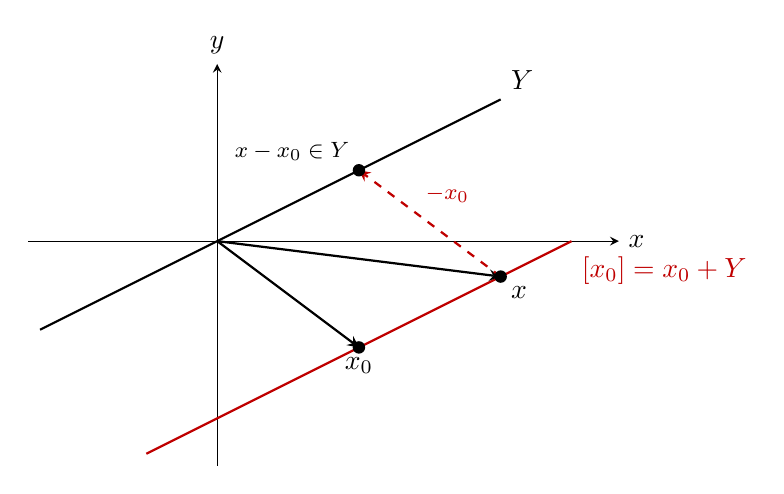
\begin{tikzpicture}[scale=1.5, >=stealth]
    \draw[->] (-1.6,0) -- (3.4,0) node[right] {$x$};
    \draw[->] (0,-1.9) -- (0,1.5) node[above] {$y$};
    \draw[thick] (-1.5,-0.75) -- (2.4,1.2) node[above right] {$Y$};
    \draw[thick, red!75!black] (-0.6,-1.8) -- (3.0,0.0) node[below right, yshift=-2pt] {$[x_0] = x_0 + Y$};
    % the vectors x_0 and x
    \draw[->, thick] (0,0) -- (1.2,-0.9) node[below] {$x_0$};
    \draw[->, thick] (0,0) -- (2.4,-0.3) node[below right] {$x$};
    % dragging x back to Y by -x_0
    \draw[->, dashed, thick, red!75!black] (2.4,-0.3) -- (1.2,0.6) node[pos=0.6, above right, font=\footnotesize] {$-x_0$};
    \fill (1.2,0.6) circle (1.5pt) node[above left, font=\footnotesize] {$x - x_0 \in Y$};
    \fill (1.2,-0.9) circle (1.5pt);
    \fill (2.4,-0.3) circle (1.5pt);
\end{tikzpicture}
